\documentclass[12pt, xcolor=table]{beamer}

\usepackage{geometry}

\usepackage{lmodern}
\usepackage[utf8]{inputenc}
\usepackage[T1]{fontenc}		
\usepackage[english]{babel}

\usepackage{siunitx}

\usepackage{xcolor, colortbl}
\definecolor{darkgreen}{RGB}{0, 155, 85}
\definecolor{elancourt}{rgb}{1,.79,.5}
\definecolor{paris}{rgb}{.84,.1,.11}
\definecolor{nantes}{rgb}{.17,.51,.73}

\renewcommand<>\cellcolor[1]{\only#2{\beameroriginal\cellcolor{#1}}}

\definecolor{LOSS35}{RGB}{255,0,0}
\definecolor{LOSS1535}{RGB}{255,122,12}
\definecolor{LOSS0515}{RGB}{255,181,12}
\definecolor{STBL}{RGB}{58,255,12}
\definecolor{GAIN0515}{RGB}{58,178,12}
\definecolor{GAIN1535}{RGB}{56,136,17}
\definecolor{GAIN35}{RGB}{50,119,16}


\usepackage{graphicx}
\usepackage{floatrow}
\usepackage[
    scriptsize,
    labelformat=empty
]{caption}

\usepackage{enumitem}

\usepackage{standalone}

\usepackage{multirow}

\usepackage{array}
\newcolumntype{x}[1]{>{\centering\let\newline\\\arraybackslash\hspace{0pt}}m{#1}}
\usepackage{booktabs}
\usepackage{makecell}

\usepackage{tikz}
\usetikzlibrary{calc, 3d, shadows, decorations, shapes, fadings, trees, backgrounds, fit}
\usepackage{pgfplots}
\usepackage{pgfplotstable}
\usepackage{forest}
\usepackage[final]{animate}

\usepackage{amsmath}
\usepackage{amsthm}
\usepackage{amsfonts}
\usepackage{amssymb}
\usepackage{mathrsfs}
\usepackage{bm}
\usepackage{bbold}
\usepackage{stmaryrd}
\usepackage{mleftright}
    
\usepackage[
    backend=biber,
    style=authoryear,
    dashed=false,
    sorting=nty,
    maxbibnames=5,
    minbibnames=5,
    maxcitenames=1,
    uniquelist=false,
    uniquename=false,
    hyperref=true,
    backref=true,
    backrefstyle=all+,
    isbn=false,
    url=false,
    doi=false
]{biblatex}
\usepackage{xpatch}

\addbibresource{references.bib}

\usepackage[acronym, toc, automake=true]{glossaries}

\usepackage{hyperref}
\hypersetup{
    pdftitle={Semantic aware quality evaluation of 3D building models},
    pdfauthor={Oussama Ennafii},
    pdfkeywords={3D urban modeling} {buildings} {quality assessment} {taxonomy} {classification} {error detection} {geometry} {aerial imagery} {Very High Spatial Resolution} {Digital Surface Model},
    pdfstartview={FitH},
    unicode=true
}

\setbeamerfont{footnote}{size=\tiny}

\tikzset{
    invisible/.style={opacity=0},
    visible on/.style={alt=#1{}{invisible}},
    alt/.code args={<#1>#2#3}{
        \alt<#1>{\pgfkeysalso{#2}}{\pgfkeysalso{#3}}
    },
}

\NewDocumentCommand{\evalat}{sO{\big}mm}{%
    \IfBooleanTF{#1}
    {\mleft. #3 \mright|_{#4}}
    {#3#2|_{#4}}%
}
\makeatletter
\newcommand{\ostar}{\mathbin{\mathpalette\make@circled\star}}
\newcommand{\make@circled}[2]{%
    \ooalign{$\m@th#1\smallbigcirc{#1}$\cr\hidewidth$\m@th#1#2$\hidewidth\cr}%
}
\newcommand{\smallbigcirc}[1]{%
    \vcenter{\hbox{\scalebox{0.77778}{$\m@th#1\bigcirc$}}}%
}
\makeatother


\usepackage[useregional]{datetime2}

\usepackage{style/glossaries}

\usetheme{ign}

\title{Semantic aware quality evaluation of 3D building models}
\subtitle{A scalable approach}
\date{\tiny \DTMdisplaydate{2020}{1}{10}{5}}
\author{
    Oussama Ennafii
}

\institute{
    PhD defense
}

\begin{document}
    \begin{frame}[plain]
        \titlepage
    \end{frame}

    \section{Introduction}
        \subsection{Context}
            \begin{frame}{Applications of \texorpdfstring{\acrshort*{acr::3d}}{3D} models}
                \framesubtitle<1>{Physical simulation}
                \framesubtitle<2>{Urban planning}
                \framesubtitle<3>{Entertainement}

                \temporal<2>{
                    \begin{figure}[H]
                        \centering
                        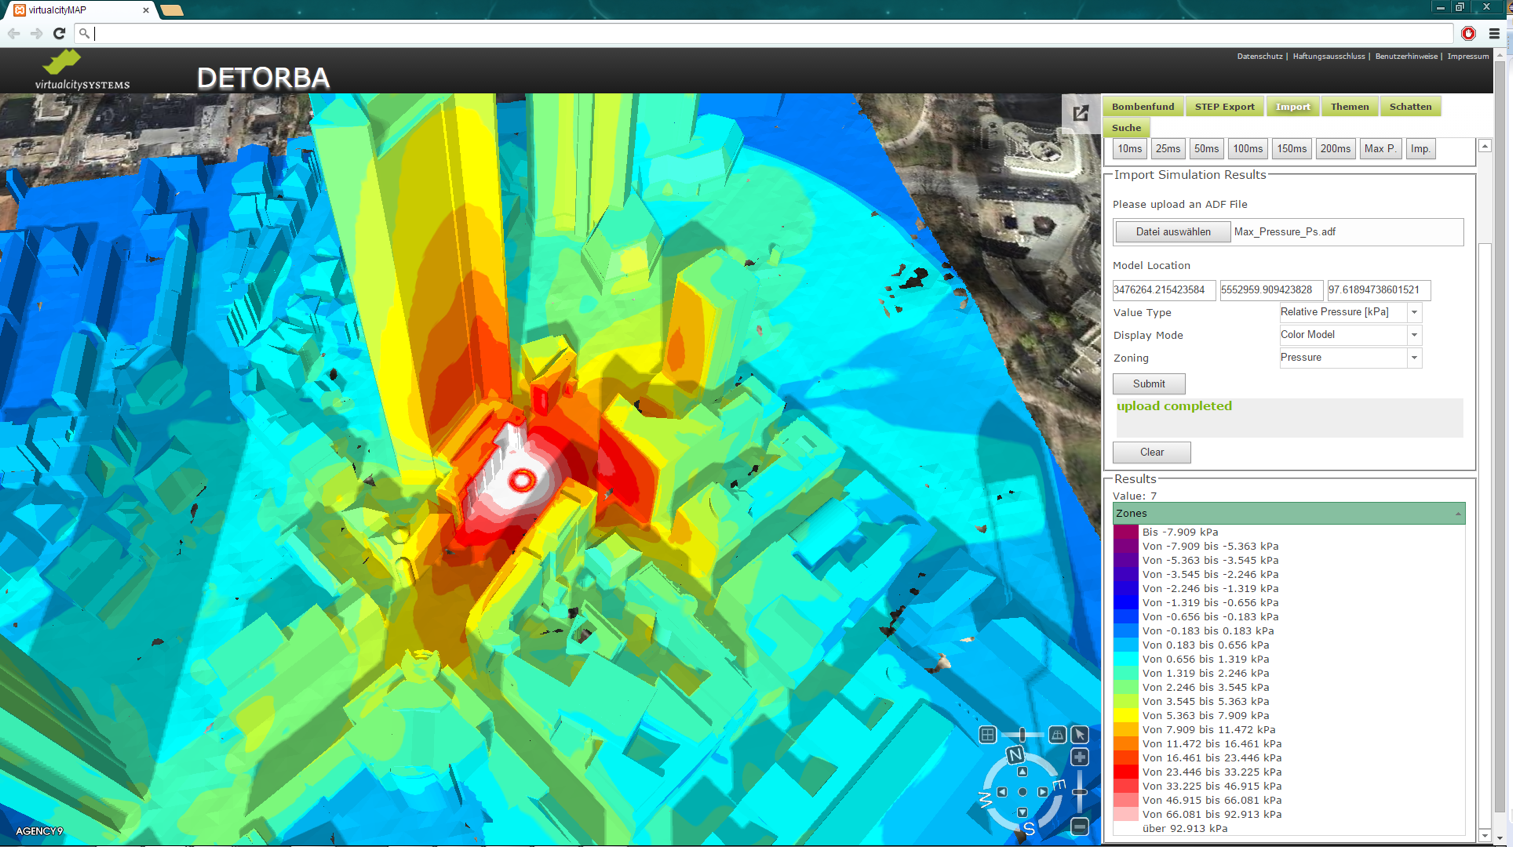
\includegraphics[width=.8\textwidth]{images/introduction/3d_model_applications/explosion_simulation}
                        \caption{Explosion simulation~\parencite{biljecki2015applications}.}
                    \end{figure}
                }
                {
                    \begin{figure}[H]
                        \centering
                        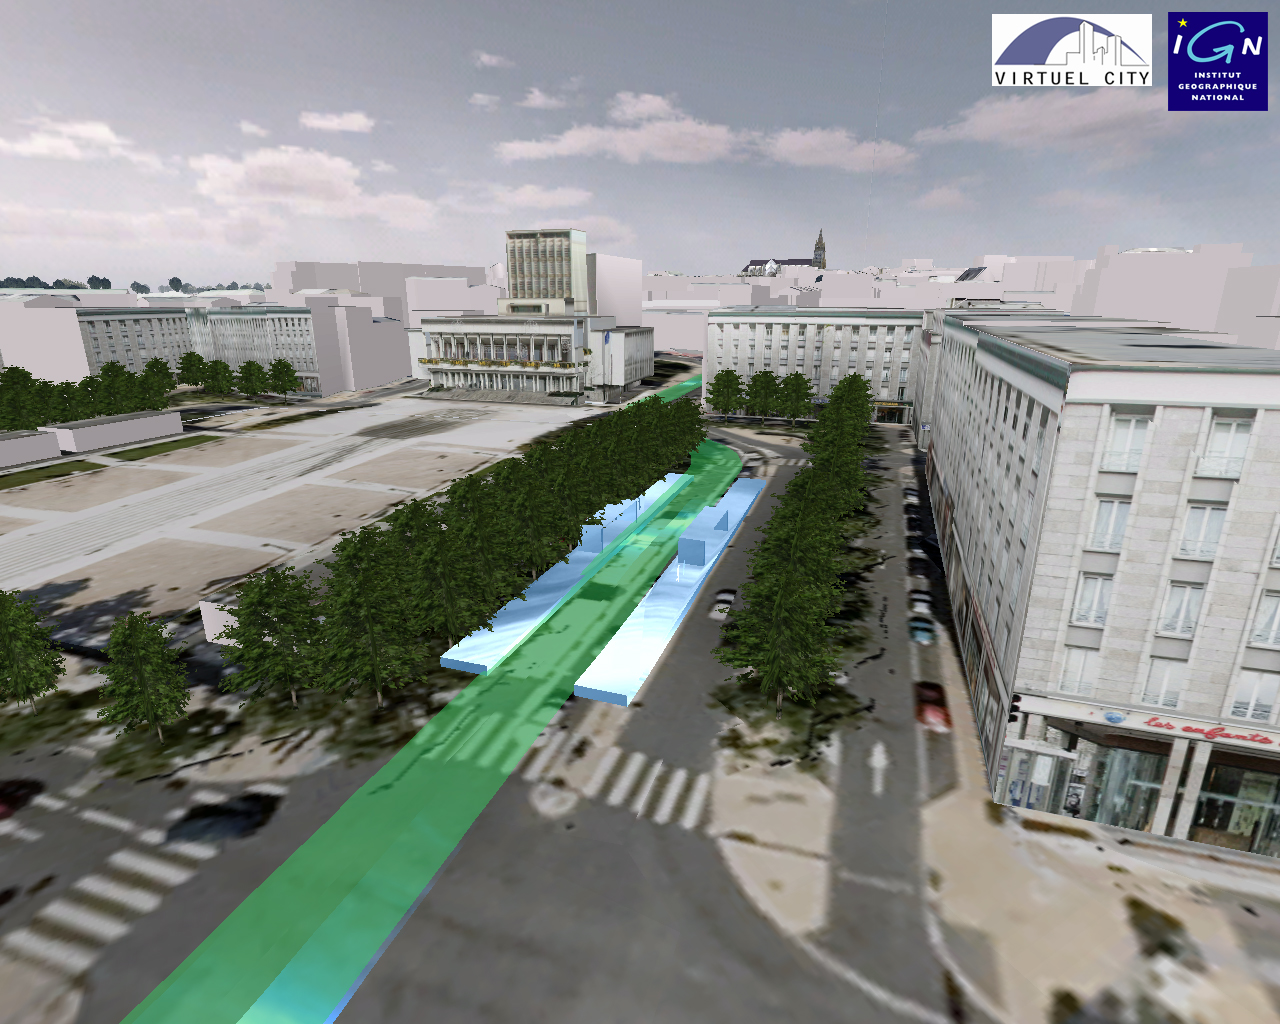
\includegraphics[width=.8\textwidth]{images/introduction/3d_model_applications/brest_tramway}
                        \caption{Example of the use of city \gls{acr::3d} models in public consultation in Brest.}
                    \end{figure}
                }
                {
                    \begin{figure}[H]
                        \centering
                        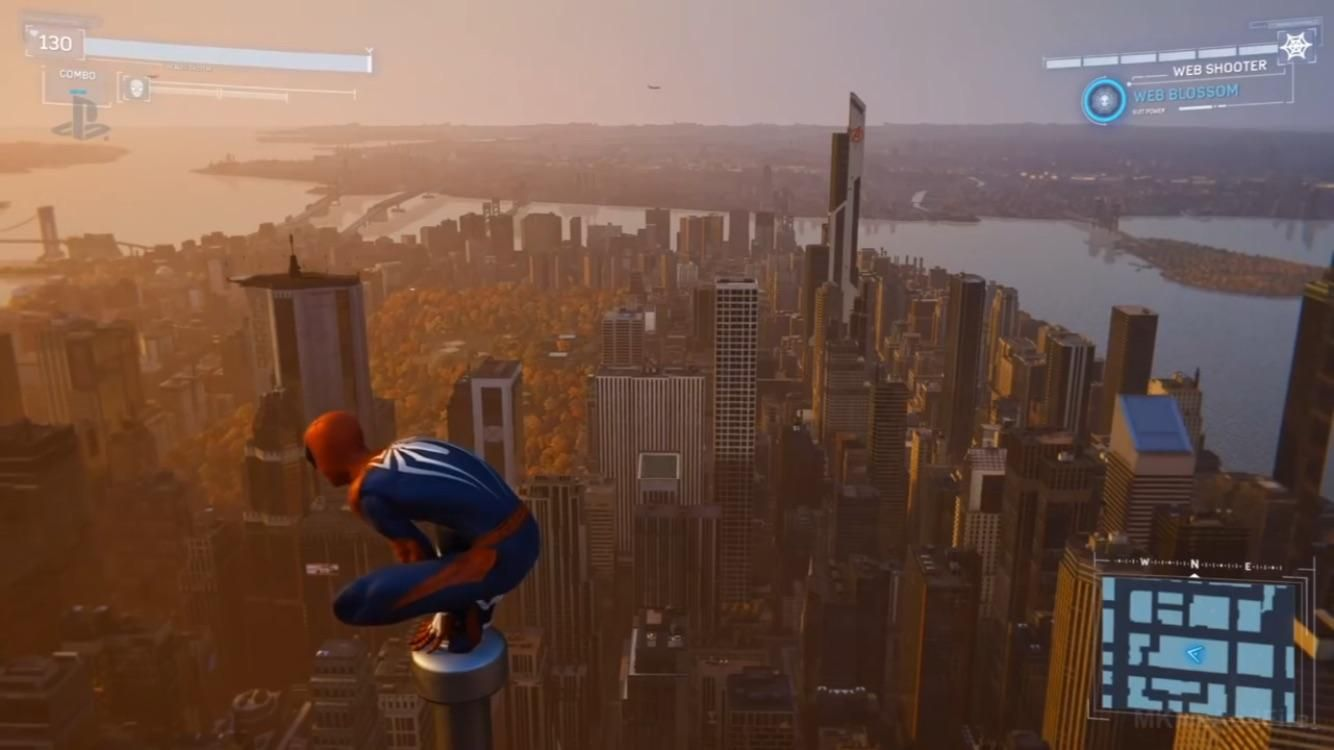
\includegraphics[width=.8\textwidth]{images/introduction/3d_model_applications/spider_man}
                        \caption{Example of the use of city \gls{acr::3d} models in video games.}
                    \end{figure}
                }
            \end{frame}

            \begin{frame}{Modeling or reconstruction}
                \begin{columns}[T]
                    \centering
                    \begin{column}{.5\textwidth}
                        \includestandalone[mode=buildnew, width=\textwidth]{figures/model_vs_mesh/mesh_model}
                        \footnotesize
                        \begin{itemize}[label=\(\blacktriangleright\), font=\color{IGNGreen}]
                            \item<1-> Building surface \underline{reconstruction}.
                            \item<2-> Geometric \underline{fidelity}.
                            \item<3-> \num{10000} facets.
                            \item<4-> Weak geometric constraints.
                        \end{itemize}
                    \end{column}
                    \begin{column}{.5\textwidth}
                        \includestandalone[mode=buildnew, width=\textwidth]{figures/model_vs_mesh/ground_truth_model_animated}
                        \footnotesize
                        \begin{itemize}[label=\(\blacktriangleright\), font=\color{IGNGreen}]
                            \item<1-> Building \underline{modeling}.
                            \item<2-> Geometric fidelity + Compacity.
                            \item<3-> \num{800} facets.
                            \item<only@4> Semantics \(\implies\) impact on geometry.
                            \item<only@5> \textit{Implicit} semantics. \phantom{on geometry}
                        \end{itemize}
                    \end{column}
                \end{columns}
            \end{frame}

            \begin{frame}{\texorpdfstring{\acrshort*{acr::3d}}{3D} model}
                \centering
                \includestandalone[mode=buildnew, width=.7\textwidth]{figures/model_information}
                
            \end{frame}

            \begin{frame}{\texorpdfstring{\acrshort*{acr::3d}}{3D} building modeling}
                \begin{figure}[H]
                    \centering
                    
\includegraphics[width=\textwidth]{images/introduction/lods_3}
                    \caption{\glspl{acr::lod} considered in the study~\parencite{biljecki2016improved}.}
                \end{figure}
            \end{frame}
        
        \subsection{Quality evaluation}
            \begin{frame}{Modeling errors}{Different point of views}
                \begin{itemize}[label=\(\blacktriangleright\), font=\color{IGNGreen}]
                    \item<1-> Errors in format: compliancy to OGC standard\footfullcite{ledoux2013validation}.
                    \item<2-> Errors in surface reconstruction\footfullcite{berger2013benchmark}.
                    \item<3-> Errors in Modeling\footfullcite{rottensteiner2012isprs}.
                \end{itemize}
            \end{frame}

            \begin{frame}{Need for semantics}
                \begin{itemize}[label=\(\blacktriangleright\), font=\color{IGNGreen}]
                    \item<1-> Modeling \(\longleftrightarrow\) compromise between:
                    \begin{itemize}[label=\(\blacktriangleright\), font=\color{IGNGreen}]
                        \item<2-> geometric accuracy;
                        \item<3-> and \textit{implicit} semantics.
                    \end{itemize}
                    \item<4-> Errors are \underline{geometric} and \underline{semantic} in nature.
                \end{itemize}
            \end{frame}

            \begin{frame}{Goal}
                \begin{itemize}[label=\(\blacktriangleright\), font=\color{IGNGreen}]
                    \item<1-> \underline{Define errors} that affects building \gls{acr::3d} models.
                    \item<2-> Design a method for \underline{error detection}.
                \end{itemize}
            \end{frame}

            \begin{frame}{Challenges}
                \begin{itemize}[label=\(\blacktriangleright\), font=\color{IGNGreen}]
                    \item<1-> Reference data are \underline{expensive}.
                    \item<2-> Large scale : small city level > \underline{\num{1000}} buildings.
                    \item<3-> \underline{Different} urban scenes \(\implies\) High \underline{heterogeneity}.
                    \item<6-> Manual evaluation: \SI[per-mode=repeated-symbol]{2}{\hour\per\km\squared\per\expert}.
                \end{itemize}
            \end{frame}
            
            \begin{frame}{State of the art}
                \centering
                \includestandalone[mode=buildnew, width=\textwidth]{figures/state_of_the_art}
            \end{frame}

            \begin{frame}{What do we want?}
                \begin{itemize}[label=\(\blacktriangleright\), font=\color{IGNGreen}]
                    \item<1-> Readily accessible reference data;
                    \item<2-> \textbf{Scalability} up to city level;
                    \item<3-> Genericity towards:
                        \begin{itemize}
                            \item<4-> modeling approach;
                            \item<5-> urban scene.
                        \end{itemize}
                    \item<6-> \textbf{Automation}: least human intervention possible.
                \end{itemize}
            \end{frame}

            \begin{frame}{Our answer}
                \begin{enumerate}[label=\arabic*), itemsep=2em]
                    \item<1-> Semantic error taxonomy;
                    \item<2-> Learning based evaluation approach;
                    \item<3-> Experimental validation.
                \end{enumerate}
            \end{frame}

    \section{Conclusion}
        \begin{frame}{Summary}
            \begin{itemize}[label=\(\blacktriangleright\), font=\color{IGNGreen}]
                \item<1-> \textbf{Hierarchical and modular} error taxonomy;
                \item<2-> \textbf{Scalable} evaluation method;
                \item<4-> Intrinsic features could be used for error prediction;
                \item<5-> Extrinsinc modalities \(\implies\) better transferability.
                \item<6-> Advanced features \(\implies\) high prediction scores.
            \end{itemize}
        \end{frame}
        \begin{frame}{Perspectives}
            \begin{itemize}[label=\(\blacktriangleright\), font=\color{IGNGreen}]
                \item<1-> Use of deep learning:
                \begin{itemize}[label=---]
                    \item Dataset augmentation $\longrightarrow$ \textbf{Simulate errors};
                    \item Semi-supervized learning.
                \end{itemize}
                \item<2-> Localizing errors: facet level.
                \item<3-> Automatic correction.
                \item<4-> Generalize to \gls{acr::lod}-3.
            \end{itemize}
        \end{frame}

    \bgroup
    \setbeamercolor{background canvas}{bg=white}

    \begin{frame}[plain]{}
        \newgeometry{top=0cm, left=0cm, right=0cm, bottom=0cm}
        \hspace{-.75cm}
        \begin{tikzpicture}
            \node (ign_logo) at (-1, 0) {
                
\includegraphics[width=1.606911447cm]{images/logos/logo-ign}
            };
            \path (ign_logo.south) node[anchor=north] (inria_logo) {
                
\includegraphics[width=1.606911447cm]{images/logos/logo-inria}
            };
            \path (inria_logo.south) node[anchor=north] (upe_logo) {
                
\includegraphics[width=1.606911447cm]{images/logos/logo-upe}
            };
            \path (ign_logo.north east) + (3, 0) node[anchor=north west] (trame) {\usebox \tramebox};
            \path (upe_logo.south west) + (0, -1.75) node[anchor=north west] (background) {
                {
                    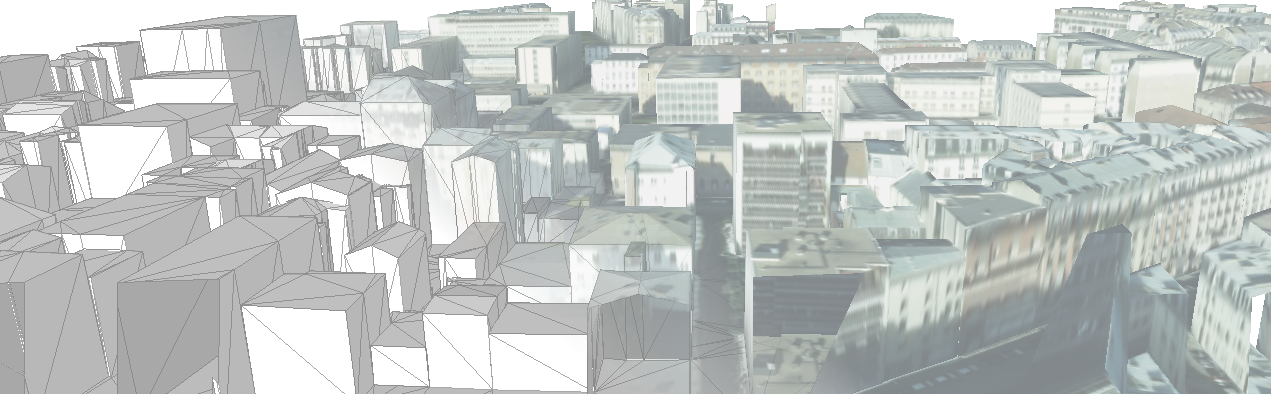
\includegraphics[width=11.5cm]{images/logos/background-50}
                }
            };
            \path (trame.west) + (2.5, -.75) node (title_box) {\usebox \titlebox};
            \path (title_box) + (0, .75) node (thanks) {
                \begin{beamercolorbox}[
                    wd=4cm,
                    sep=8pt
                ]{title page header}
                    \usebeamerfont{title}
                    \begin{center}
                        Thank you for your attention!
                    \end{center}
                \end{beamercolorbox}
            };
            \path (background.north) node[anchor=north] (author) {
                \begin{beamercolorbox}[
                    wd=4cm,
                    sep=8pt
                ]{author}
                    \usebeamerfont{author}
                    \begin{center}
                        \insertauthor\par
                    \end{center}
                \end{beamercolorbox}
            };
            \end{tikzpicture}
        \restoregeometry 
    \end{frame}
    \egroup

    \begin{frame}{Graph kernels}
        \centering
        \includestandalone[mode=buildnew, width=\textwidth]{figures/features/graph_kernels/kernels_menu_all}
    \end{frame}

    \begin{frame}{Random walk on graphs}
        \begin{figure}[H]
            \caption{Random walk on graph \(G\).}
            \alt<1>{
                \centering
                \animategraphics[autoplay, loop, width=.45\textwidth]{25}{figures/features/graph_kernels/drunk_man/drunk_man-}{0}{72}
                \includestandalone[mode=buildnew, width=.45\textwidth]{figures/features/graph_kernels/random_walk}
            }{
                \centering
                \includestandalone[mode=buildnew, width=.45\textwidth]{figures/features/graph_kernels/random_walk}
            }
        \end{figure}
        \begin{itemize}[label=\(\blacktriangleright\), font=\color{IGNGreen}]
            \item<4-> Described \(\longrightarrow\) normalized adjacency matrix \(P\);
            \item<5-> \(P\) as a feature vector \only<6->{ \(\longrightarrow\) \alert<6->{No};}
            \item<7-> \(P\) is not \underline{invariant} to:
            \begin{itemize}[label=-]
                \item<8-> permutations;
                \item<9-> graph size.
            \end{itemize}
            \item<10-> Kernel trick \(\longrightarrow\) compare graphs instead.
        \end{itemize}
    \end{frame}

    \begin{frame}{Random walk based}
        \framesubtitle<1-4>{Random walk kernel}
        \framesubtitle<5-13>{Multiscale Laplacian kernel}
        \framesubtitle<14->{Propagation kernel}
        \only<1-4>{
            \begin{columns}[T]
                \centering
                \begin{column}{.4\textwidth}
                    \centering
                    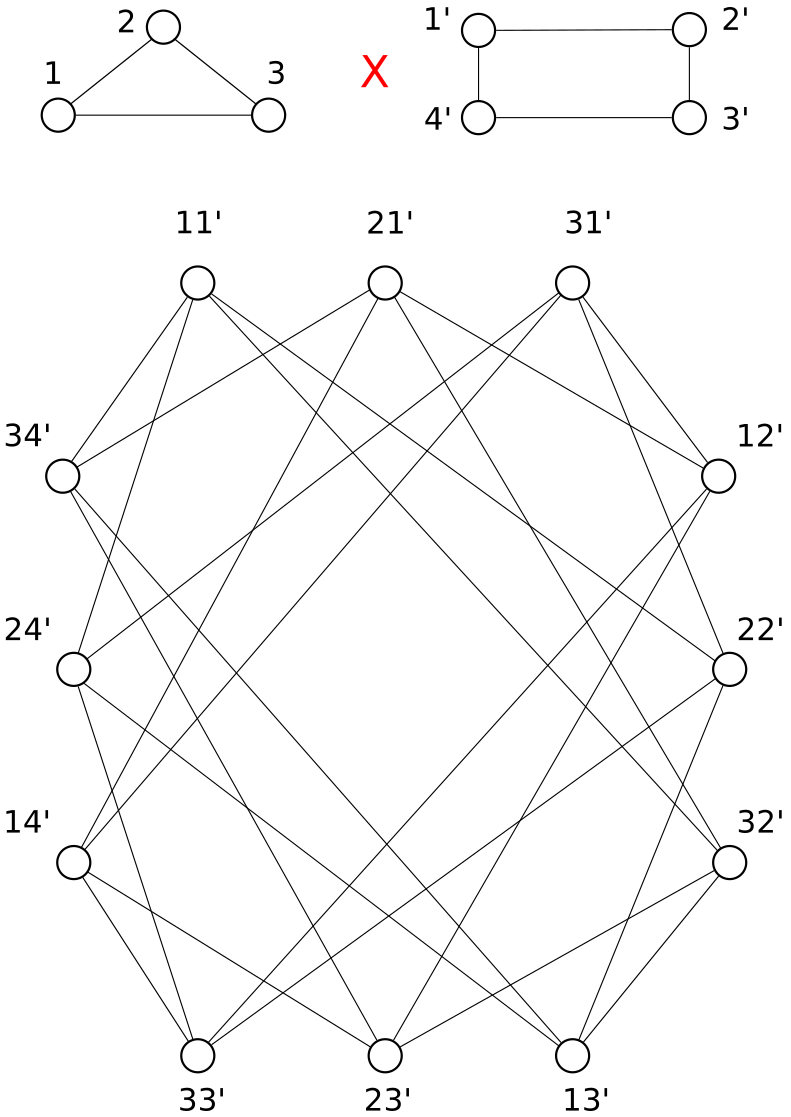
\includegraphics[width=\textwidth]{images/related_work/direct_product_graphs}
                \end{column}
                \begin{column}{.56\textwidth}
                    \centering
                    \begin{itemize}[label=\(\blacktriangleright\), font=\color{IGNGreen}]
                        \item<2-> Quadratic form with \(P_{\times}\) \(\implies\) \underline{invariance} to:
                            \begin{itemize}[label=-]
                                \item<3-> permutation;
                                \item<4-> graph size;
                            \end{itemize}
                    \end{itemize}
                \end{column}
            \end{columns}
        }
        \only<5-13>{
            \vfill
            \begin{itemize}[label=\(\blacktriangleright\), font=\color{IGNGreen}]
                \item<5-> \(G\) \(\longleftrightarrow\) Variance matrix of a \underline{Gaussian distribution}.
                \item<6-> Compare graphs \(\longleftrightarrow\) Compare probabilities.
                \item<7-> Adapted to be:
                \begin{itemize}[label=\(\blacktriangleright\), font=\color{IGNGreen}]
                    \item<8-> permutation and size invariant \(\longrightarrow\) \only<9->{linear embedding;}
                    \item<10-> node attribute aware \(\longrightarrow\) \only<11->{vertex kernel Gram matrix;}
                    \item<12-> scalability \(\longrightarrow\) \only<13->{kernel between pyramid of subgraphs.}
                \end{itemize}
            \end{itemize}
            \vfill
        }
        \only<14->{
            \begin{itemize}[label=\(\blacktriangleright\), font=\color{IGNGreen}]
                \item<14-> Nodes are \underline{Gaussian mixtures} of other nodes;
                \item<15-> Propagate mixture \underline{coefficients} using \(P\);
                \item<16-> Probability distributions are \underline{hashed} \(\longrightarrow\) \onslide<17->{graph feature vector}.
            \end{itemize}
        }
    \end{frame}

    \begin{frame}{Random walk}{Tottering}
        \begin{figure}[H]
            \centering
            \includestandalone[mode=buildnew, width=.5\textwidth]{figures/features/graph_kernels/tottering}
        \end{figure}
        \begin{itemize}
            \item Tottering \(\longleftrightarrow\) cycles;
            \item \textcolor{purple}{Central} nodes are overrepresented;
            \item \textcolor{purple!30}{Isolated} nodes are less visited.
        \end{itemize}
    \end{frame}

    \begin{frame}{Path based}{Graph Hopper kernel}
        \begin{figure}[H]
            \centering
            \includestandalone[mode=buildnew, width=\textwidth]{figures/features/graph_kernels/graph_hopper}
        \end{figure}

        \begin{itemize}[label=\(\blacktriangleright\), font=\color{IGNGreen}]
            \item<2-> Use \underline{paths} instead (no cycles);
            \begin{itemize}[label=\(\blacktriangleright\), font=\color{IGNGreen}]
                \item<3-> Compare same length paths.
                \item<7-> Hop and compare vertex attributes \(\longrightarrow\) base kernel.
                \item<11-> Sum over all vertex comparisons \(\longrightarrow\) \underline{invariance}.
            \end{itemize}
        \end{itemize}
    \end{frame}

    \begin{frame}{Lov\'asz/\texorpdfstring{\acrshort*{acr::svm}}{SVM} kernel}
        \begin{itemize}[label=\(\blacktriangleright\), font=\color{IGNGreen}, itemsep=2em]
            \item<1-> Lov\'asz number \(\vartheta\left(G\right)\):
            \begin{itemize}[label=\(\blacktriangleright\), font=\color{IGNGreen}]
                \item<2-> graph invariant;
                \item<3-> smallest cone containing the orthonormal representation of \(G\).
            \end{itemize}
            \item<4-> Compare graphs \(\longleftrightarrow\) Compare Lov\'asz number of their subgraphs.
            \item<5-> \(\vartheta\left(G\right)\) not easy to compute \(\longleftrightarrow\) Approximation with \gls{acr::svm}kernel.
        \end{itemize}
    \end{frame}


    \begin{frame}{\texorpdfstring{\acrshort*{acr::scatnet}}{ScatNet} structure}
        \centering
        \includestandalone[mode=buildnew, height=.8\textheight]{figures/scattering_network_animated}
    \end{frame}

\end{document}
